%% Copernicus Publications Manuscript Preparation Template for LaTeX Submissions
%% ---------------------------------
%% This template should be used for copernicus.cls
%% The class file and some style files are bundled in the Copernicus Latex Package, which can be downloaded from the different journal webpages.
%% For further assistance please contact Copernicus Publications at: production@copernicus.org
%% https://publications.copernicus.org/for_authors/manuscript_preparation.html


%% Please use the following documentclass and journal abbreviations for preprints and final revised papers.

%% 2-column papers and preprints
\documentclass[hess, manuscript]{copernicus}



%% Journal abbreviations (please use the same for preprints and final revised papers)


% Advances in Geosciences (adgeo)
% Advances in Radio Science (ars)
% Advances in Science and Research (asr)
% Advances in Statistical Climatology, Meteorology and Oceanography (ascmo)
% Annales Geophysicae (angeo)
% Archives Animal Breeding (aab)
% ASTRA Proceedings (ap)
% Atmospheric Chemistry and Physics (acp)
% Atmospheric Measurement Techniques (amt)
% Biogeosciences (bg)
% Climate of the Past (cp)
% DEUQUA Special Publications (deuquasp)
% Drinking Water Engineering and Science (dwes)
% Earth Surface Dynamics (esurf)
% Earth System Dynamics (esd)
% Earth System Science Data (essd)
% E&G Quaternary Science Journal (egqsj)
% European Journal of Mineralogy (ejm)
% Fossil Record (fr)
% Geochronology (gchron)
% Geographica Helvetica (gh)
% Geoscience Communication (gc)
% Geoscientific Instrumentation, Methods and Data Systems (gi)
% Geoscientific Model Development (gmd)
% History of Geo- and Space Sciences (hgss)
% Hydrology and Earth System Sciences (hess)
% Journal of Bone and Joint Infection (jbji)
% Journal of Micropalaeontology (jm)
% Journal of Sensors and Sensor Systems (jsss)
% Magnetic Resonance (mr)
% Mechanical Sciences (ms)
% Natural Hazards and Earth System Sciences (nhess)
% Nonlinear Processes in Geophysics (npg)
% Ocean Science (os)
% Primate Biology (pb)
% Proceedings of the International Association of Hydrological Sciences (piahs)
% Scientific Drilling (sd)
% SOIL (soil)
% Solid Earth (se)
% The Cryosphere (tc)
% Weather and Climate Dynamics (wcd)
% Web Ecology (we)
% Wind Energy Science (wes)


%% \usepackage commands included in the copernicus.cls:
%\usepackage[german, english]{babel}
%\usepackage{tabularx}
%\usepackage{cancel}
%\usepackage{multirow}
%\usepackage{supertabular}
%\usepackage{algorithmic}
%\usepackage{algorithm}
%\usepackage{amsthm}
%\usepackage{float}
%\usepackage{subfig}
%\usepackage{rotating}


\begin{document}

\title{TopoCLIM: Rapid topography based downscaling of regional climate model output in complex terrain 
%Topographic based downscaling of climate time series in data sparse regions using quantile mapping
}


% \Author[affil]{given_name}{surname}

\Author[1]{Joel}{Fiddes}
\Author[2]{Kristoffer}{Aalstad}
\Author[1,3]{Michael}{Lehning}


\affil[1]{WSL Institute for Snow and Avalanche Research SLF, Davos, Switzerland}
\affil[2]{Department of Geosciences, University of Oslo, P.O. Box 1047, Blindern, 0316 Oslo, Norway}
\affil[3]{CRYOS, School of Architecture, Civil and Environmental Engineering, Ecole Polytechnique Fédérale de Lausanne, Lausanne, Switzerland}

%% The [] brackets identify the author with the corresponding affiliation. 1, 2, 3, etc. should be inserted.

%% If an author is deceased, please mark the respective author name(s) with a dagger, e.g. "\Author[2,$\dag$]{Anton}{Aman}", and add a further "\affil[$\dag$]{deceased, 1 July 2019}".

%% If authors contributed equally, please mark the respective author names with an asterisk, e.g. "\Author[2,*]{Anton}{Aman}" and "\Author[3,*]{Bradley}{Bman}" and add a further affiliation: "\affil[*]{These authors contributed equally to this work.}".


\correspondence{Joel Fiddes (joel.fiddes@slf.ch)}

\runningtitle{Downscaling climate time series in data sparse regions}

\runningauthor{TEXT}





\received{}
\pubdiscuss{} %% only important for two-stage journals
\revised{}
\accepted{}
\published{}

%% These dates will be inserted by Copernicus Publications during the typesetting process.


\firstpage{1}

\maketitle



\begin{abstract}
This study describes and evaluates a new downscaling scheme which specifically addresses the need for hillslope scale atmospheric forcing timeseries for modeling the local impact of regional climate change projections on the land surface in complex terrain. The method has a global scope and is able to generate the full suite of model forcing variables required for hydrological and land surface modeling at hourly timesteps. 

It achieves this by utilising the previously published TopoSCALE scheme \citep{Fiddes2014-wt} to generate a synthetic observation of current climate at hillslope scale, while accounting for a broad range of surface-atmosphere interactions. These synthetic observations are then used to debias (downscale) CORDEX climate variables using the quantile mapping method. A further temporal disaggregation step produces sub-daily fields. This approach has the advantages of other empirical-statistical methods, namely speed of use, while avoiding the need for ground data, which is often limited. It is therefore a suitable method for a wide range of remote regions where ground data is absent, incomplete, or not of sufficient length. The approach is evaluated using a network of high elevation stations across the Swiss Alps and a test application of modelling climate change impacts on Alpine snow cover is given. 
\end{abstract}





\introduction  %% \introduction[modified heading if necessary]

Climate change has, and will continue to cause significant changes in the global cryosphere with increasing impacts likely in a wide range of domains \citep{hock2019high}. Where observational records of sufficient length exist we are able to quantify these changes. Such records are often curated as part of national or international networks e.g. the World Meteorological Organisation's Global Cryosphere Watch, World Glacier Monitoring Service or the Global Climate Observing System. However, such locations are globally sparse, with particular observational gaps in remote regions due to technical difficulties and resources required to maintain monitoring infrastructure. 

In order to obtain possible scenarios of future conditions we are reliant on climate models. However, for meaningful impact studies climate time-series are often required at higher spatial and temporal resolutions than currently available from Global or even Regional Climate Models (GCMs/ RCMs). This is especially the case in heterogeneous terrain such as mountain regions where topographic variability is high over short horizontal distances. Various methods of downscaling can be utilised to achieve this goal. Dynamical downscaling typically applies an RCM or numerical weather prediction model (e.g. WRF) at high resolution over a limited area in order to obtain more detailed process representation. This requires no additional data beyond a boundary forcing, yet is computationally costly (normally a super-computing centre is required) and therefore generally applied to limited domains and/or time periods. In addition, an extensive set of boundary fields are required in order to set up a run that are not normally available via standard distribution portals such as Earth System Grid Federation (ESGF), further complicating possible studies. Empirical-statistical downscaling (ESD) approaches are typically computationally cheap to run yet require extensive and robust ground observations that are often either not available, of uncertain quality, or distributed unequally according to important gradients such as elevation. In addition, timeseries from many stations are not available at climate timescales - typically 30 years \citep{Arguez2011-qv}, rendering the application of ESD methods problematic. Furthermore, many modern physically based impact models require a full suite of forcing variables to drive them, usually at sub-daily time-steps. Such requirements are rarely met by initiatives that have provided input for impact studies \citep{Michel2021-mb}. It is increasingly recognized that analysis of extremes, and not just mean values, is required to fully quantify the impact of climate change \citep{Katz1992-xb}. By definition this requires high temporally resolved forcings, as climatic extremes often occur over short timescales e.g daily maximum temperature or storm peak that require sub-daily simulations.

Climate model timeseries, even from the latest generation of RCMs, typically exhibit bias (systematic deviations) when evaluated against observations \citep{Ivanov2018-vz, Kotlarski2014-rf}. These biases need to be corrected before climate timeseries can be used to force a locally applied impact model \citep{Wood2004-vu}. However, in impact studies we are typically interested in a climate change signal (CCS) which is a quantitative measure of the difference between a future climate statistic and historical reference period \citep{Themesl2012-um}. Bias correction (BC) can modify the CCS \citep{Ivanov2018-vz, Themesl2012-um}  which has been a subject of discussion and often seen as a deficiency in BC methods \citep{Hempel2013-sj}. However, it is recognised that model biases typically do not cancel out in the calculation of a CCS and therefore its modification under BC has been interpreted recently as an enhancement rather than a deficit, particularly in intensity dependent biases which characterise variables such as precipitation \citep{Gobiet2015-yw}.

There are a wide range of BC methods \citep{Gutmann2014-dq} with perhaps the most established and widely used being quantile mapping (QM) which has been shown to be most performant in comparison studies \citep{Teutschbein2013-nn, Jakob_Themes_l2011-xt} and found to cope best with with non-stationary conditions - a key assumption of climate model bias correction. It is also one of the few methods able to correct wet day frequency and intensity.  QM is a distribution based BC method that removes quantile dependent biases with respect to a reference period \citep{Ivanov2017-lt}, it therefore corrects the variance and not just the mean. It should be noted that if the the climate variable and reference are at the same spatial scale a pure bias correction is applied, whereas if the reference is at a finer scale (e.g. a meteorological station) then an implicit downscaling is achieved, making it also a class of empirical-statistical downscaling (ESD) methods.

While concerns over the deterministic nature of QM \citep{Maraun2013-gq} and effect on multi-day statistics \citep{Addor2014-ew}  are acknowledged, it is widely accepted to be a pragmatic approach to satisfy the requirements of impact models \citep{Rajczak2016-jk} with deficits shared by all statistically-based methods. A useful overview of the issues involved with respect to impact modelling can be obtained from \citet{Stocker_TF}.

%The assumption that bias structure is stationary through time is key to all BC methods and found to cope best with with non-stationary conditions - a key assumption of climate model bias correction

% bad link here
All ESD/BC methods require climate scale timeseries of observations (typically 30 years), in remote regions lacking sufficient historical observations this requirement can be difficult to achieve. Atmospheric reanalysis data-sets have been proposed as a means to compensate for missing or incomplete observations \citep{Cao2019-wx, Fiddes2014-wt} in order to provide a "best-guess" of the current state. Moreover, global reanalysis datasets can form the basis for impact studies with a global consistency. %However, we know these may also exhibit bias in some respects \citep{Orsolini2019-vo,Wang2019-px,Liu2019-fk}, further complicating our ability to quantify the impacts of climate change.

In this study we address the problem of impact-model ready climate timeseries with a new modelling framework called "TopoCLIM". We use the latest ECMWF global reanalysis dataset ERA5 together with the downscaling method TopoSCALE \citep{Fiddes2014-wt} to provide a robust assessment of local-scale meteorological forcing for the reference period. Using these pseudo-observation we are able to debias climate timeseries in regions lacking ground observations. Furthermore, this method provides a full suite of forcing data required to run a numerical model at sub-daily timesteps. 

By coupling this to the subgrid spatial scheme \citep{Fiddes2012-td} and the snow model FSM \cite{Essery2015-jv}, we demonstrate the ability of this scheme to efficiently generate high resolution (100~m) climate change maps of snow cover over the entire Swiss Alps. We test this scheme both with a detailed evaluation at the Weissfluhjoch meteorological station, and across the Swiss network of high elevation stations (IMIS) which has a large spatial support. %Finally we producing future snow-cover maps at 100m for the entire Swiss Alps, 1980-2100.  


%The contribution of the method outlined here is the ability to generate climate timeseries capable of forcing a numerical model at any point globally. 
%Efficiently means the code is designed to run either on an institutional cluster or even a personal laptop with runtimes normally measured in minutes to hours. Of course this depends on cluster v PC and size of domain.
%However, in many regions where we are lacking current.
%Existing climate products eg CH2018
%Existing tools \citep{parey2019}


\section{Methods}

\subsection{Overview}
The scheme is implemented in Python with several specific sub-routines implemented in R (e.g. the quantile mapping package). An overview of the processing pipeline is given in Figure 2 and can be summarised as a three-step process: (1) A quasi-physical topography-based downscaling method TopoSCALE \citep{Fiddes2014-wt} generates hillslope scale (defined by the DEM resolution) forcing time-series for the reference period from the ERA5 reanalysis. 
%We debias the current period using a data assimilation scheme based on a particle batch smoother \citep{Fiddes2019-vy} and MODIS snow cover information.  
(2) the BC method quantile mapping \citep{Gudmundsson2012-kn} is used to statistically downscale (debias) a climate time series at the given point for which we now have a reference from downscaled ERA5 forcing. (3) a disaggregation scheme \citep{Forster2016-xx} generates hourly climate timeseries based on observed sub-daily distributions of meteorological variables. We demonstrate this approach by downscaling CORDEX RCM data at both hillslope scale and additionally generalising this to a map product using the subgrid scheme, TopoSUB \citep{Fiddes2012-td}. The overall philosophy of this approach is to develop methods that are global in application and therefore can be used in data-poor regions, are efficient to run and repeat (ability to be experimental), and yet address the key drivers of climate-surface variability in complex terrain.

\subsection{Preprocessing}
The CORDEX data download is achieved using a custom tool built around the ESGF python client. This is not a trivial task due to the large data volumes involved and variable uptime of data nodes. %These issues are handled by the module 'esgf\_get.py' in the tclim package. 
All preprocessing steps of raw CORDEX data, such as concatenating NetCDF time series, extracting region of interest and regridding from rotated pole projections, was accomplished using standard tools from the Climate and Data Operators (CDO) toolkit. The CDO tools are incorporated into the preprocessing module of TopoCLIM and not used as standalone command line tools - enhancing the ease of use of the processing pipeline. As downloads are done by variable, it is possible that the full set of required forcing variables are not available for a given CORDEX model chain. If this is the case the model chain is excluded from any further processing. 

Climate model calendars are often simplified for numerical reasons and are inherited from the parent GCM, these need to be correctly handled to produce comparable timeseries. Three calendars exist in the CORDEX data used here: "360-day" (every month is 30 days long), "365-day" (no leap year), and "standard" (complete Gregorian calendar). We convert all calendars to "standard" by linearly scaling dates to the standard Gregorian calendar and then gap filling missing data by linear interpolation. For example conversion from a "360-day"  to a "standard" calendar, the output from the linear scaling will result in a 365 day timeseries (in the case of non-leap year) and be missing the following dates: January 31st, March 31st, June 1st, July 31st, September 31st and November 30th. In a second step these dates are linearly gap-filled.

\subsection{Spatial downscaling of observations}
ERA5 reanalysis \citep{Hersbach2020-ze} “observations” are downscaled using the TopoSCALE scheme \citep{Fiddes2014-wt} to be used as the reference data in the bias correction. We acknowledge that reanalyses are not true observations \citep{Parker2016-qq}, yet by assimilating an extensive set of observations into an NWP model, reanalysis are often considered to give the best possible view of the global climate \cite{Dee2014-de}. TopoSCALE performs a 3D interpolation of atmospheric fields available on pressure levels, to account for time varying lapse rates, and a topographic correction of radiative fluxes. These include a cosine correction of incident direct shortwave radiation on a slope, adjustment of diffuse shortwave and longwave radiation by the sky view factor, and elevation correction of both longwave and direct shortwave. It has been extensively tested in various geographical regions and applications e.g. permafrost in the European Alps \citep{Fiddes2015-lx}, Northern hemisphere permafrost \citep{tc-9-1303-2015}, Antarctic permafrost \citep{Obu2020-ai}, Arctic snow cover \citep{Aalstad2018-vq}, Alpine snow cover \citep{Fiddes2019-vy}. This approach enables us to provide a climate length pseudo-observation timeseries globally, while accounting for the main topographic effects on atmospheric forcing. We call this product T-MET throughout the text.



%and used to quantile map daily climate data using the historical CORDEX period that overlaps with OBS (1980-2005).

%\subsection{Debiasing observations}
%While we assume OBS are a reasonable representation of near surface conditions this is not necessarily so as biases in ERA5 are well documented (cite) and spatially varying, largely in line with the surface observation network. One of the largest and most critical uncertainties (at least for glacio-hydrological applications), is precipitation. To address this issue in forcing uncertainty, various data assimilation (DA) strategies have been proposed (cite). In particular in the field of snow modelling a range of snow reanalysis tools have been developed (cite) and we use here the implementation of \citet{Fiddes2019-vy} based upon the work of \citep{Margulis2015-fw}. A brief overview is provided here but the reader is directed to the original publication for further details and evaluation of the method. It uses a particle batch smoother (PBS) DA algorithm to assimilate timeseries of fractional snow covered area (fSCA) from the MODIS satellite snow-cover product (cf. Section 3.5). The general methodology is (i) generate an ensemble (in PBS terminology, "particles") of simulations by perturbing forcing variables according to assumed prior distributions; (ii) the observed fSCA depletion curve for the given hydrological year and its assumed error structure is then used to constrain the particles through the PBS analysis, which computes a weighting for each particle; (iii) the constrained posterior is obtained by apllying these weights to the particles. 

\subsection{Quantile mapping}
We use the R package QMAP for this purpose \citep{Gudmundsson2012-kn}. \cite{Gudmundsson2012-kn} compared different implementations of QM for daily precipitation data and found that a non-parametric empirical approach (as implemented in the cited package) outperforms implementations relying on theoretical distributional assumptions.
While quantile mapping ensures that quantile biases are corrected in the CDF it does not account for temporally varying bias. It is therefore well suited to air temperature where we can be reasonably sure that winters are cold and summers hot, at least in mid to high latitudes. However, with precipitation intra-annual distribution can be biased while the CDF may look reasonable (e.g. wet and dry season timing could be shifted). We address this with a two step approach called QMAP\_MONTH. We split the data according to 12 temporal subsets corresponding to the months of the calendar year and run the QM algorithm on each subset, computing QM parameters separately for each month. These are applied throughout the historical and climate time series at the appropriate months. Similar approaches have been used successfully in other studies e.g. \citet{Hanzer2018-tz}. 

\subsection{Temporal downscaling of observations}
The final step in preparing the climate forcing is a temporal disaggregation to generate required sub-daily fields. Original hourly resolution T-MET are used to temporally disaggregate the downscaled (quantile mapped) daily climate timeseries. An adapted version of the Melodist package is used for this purpose \citep{Forster2016-xx}. This disaggregates daily data based on observed sub-daily distributions. It should be noted that this assumes sub-daily distributions are stationary in a future climate, which quite possibly is not the case. However a greater source of uncertainty likely exists in the ability of ERA5 to reproduce short timescale local weather patterns which require convection resolving model resolutions \citep{Liu2017-md} and appropriate physics. %What we in effect do here is to consider how daily extreme values look in the future once scaled by the information we have from daily RCM data.

\subsection{Simulation and maps}
We use the Factorial Snow Model (FSM) model \citep{Essery2015-jv} to simulate the snow cover and TopoSUB \citep{Fiddes2012-td} to spatialise results to a 2D map. Briefly, TopoSUB is a topographic sampling scheme that reduces distributed modelling problems that explicitly model individual pixels to a lumped model several orders of magnitude smaller while considering the full range of topographic heterogeneity that exists, by splitting the model domain into clusters consisting of pixels with similar terrain parameters. In this way it is possible to produce high resolution maps (e.g. DEM resolution) over large (regional) modelling domains, while explicitly including the drivers of surface-atmosphere processes.
The scheme is implemented on an HPC cluster for efficiency in an "embarrassingly parallel" sense i.e. no communication required between compute nodes. Typical setups use 100 nodes with run-times measured in minutes for full 1980-2100 runs. The scheme also has a desktop mode which typically utilises 8 cores and typical runs will require a few hours. These "benchmarks" are provided merely to give the reader an order-of-magnitude idea of how resource intensive this scheme is.

\subsection{Treatment of glaciers}
Glacier zones are typically masked in studies of seasonal snow unless a glacier layer is explicitly accounted for in the model. 
%However, we think it is useful to show the climate-viable glacier accumulation zone i.e. the region under a steady state climate where glaciers would develop in the model due to non-melt of seasonal snow at the end of the summer and accumulates from year to year. This defines an accumulation zone only of course and ignores all glacier dynamics. We mask out pixels that do not melt out in the analysis - indicating glacier accumulation regions and further analyse the evolution of these "accumulation zones" in the climate runs.
In this study, however, we wanted to highlight and track changes in the glacier accumulation zones. These zones are areas where the annual surface mass balance is positive, leading to the formation or growth of glaciers. With our framework we are able to identify such zones, but we ignore glacier dynamics so we are not able to map the evolution of glaciers.
%Additionally, this only considers the meteorological forcing and topographical position (which defines the meteo forcing through TopoSCALE) and does not consider changing ground heat-fluxes.





\section{Study region and data}
\subsection{Model domain}
We consider two scales in this study (a) point-scale (meteorological station, Weissfluhjoch and IMIS network) and (b) regional (Swiss Alps), in order to illustrate typical applications of the scheme. A map of the study region and the location of the stations we used is given in Figure 1.

\subsection{Climate data}
The basic forcing comes from the regional climate model project CORDEX EUR-44 product \citep{Jacob2014-yw} at nominal resolution of 44\unit{km}. The 44\unit{km} product was chosen over the 22\unit{km} product as this had many more model chains available. The EURO domain also has an 11\unit{km} product but this is not available globally, and therefore not fit for the purpose of this study. Data was retrieved from the ESGF using an API and automated python based tool developed in this study. This is an important step as the number of file downloads are large with dimensions being $\text{models}\times\text{variables}\times\text{scenarios}\times\text{time periods}$
and the fact that the ESGF consists of a distributed set of data nodes with variable uptime, further complicates the download process. 
%Therefore we developed a tool based on the ESGF python API which simplified data retrieval and management. 
We use daily data to force the scheme and retrieve historical data plus projections from two climate change scenarios, RCP2.6 ( a "very stringent" pathway, RCP2.6 requires that  $\text{CO}_2$ emissions start declining by 2020 and go to zero by 2100) and RCP8.5 (emissions continue to rise throughout the 21st century). A full description of CORDEX datasets and models used is given in Table 2. Daily data was chosen for the method (therefore requiring a temporal disaggregation step) as limited number of model chains are available at sub-daily resolutions. This is particularly the case outside of the EURO domain where use-cases for this method are envisaged. A higher number of model chains increases confidence in our results, by improved quantification of inter-model variability. 

\subsection{Reanalysis data}
We use ECWMF's latest reanalysis product ERA5 \citep{Hersbach2020-ze}, which uses IFS 41r2 version of the ECMWF NWP model. ERA5 represents an evolution over its predecessor, ERA-Interim, by increasing the model spatial resolution to 30\unit{km}, temporal resolution to hourly and the vertical model levels to 137. These are downscaled for the purpose of bias correction using the TopoSCALE scheme \citep{Fiddes2014-wt} as described above (cf. Methods). %We call these synthetic obs (T-MET) to acknowledge they are not true observations but arguably the best option for climate scale studies.

\subsection{Topography}
NASA's SRTM-3 90\unit{m} digital elevation model (DEM) is used as a topographical surface for TopoSCALE downscaling routines. Slope, aspect and sky-view factor (the portion of the sky hemisphere that is visible for a given DEM pixel) are derived \citep{Dozier1990-jp}. A higher resolution DEM may also be used but likely does not add value as processes such as wind transport that operate on these scales are not included in the model \citep{Mott2018-pt}. Importantly, higher resolution does not necessarily increase runtime either in point mode (trivially) or in spatial mode where the run-time in the main programme modules is related to number of TopoSUB clusters. Additionally, the scheme is designed to scale well by generating cluster forcings through array computations.

%\subsection{Assimilated fSCA observations} % need to eddit!! FROM DA paper!!

%We assimilate fSCA retrievals obtained from version 6 of the level 3 daily MODIS snow-cover product from the Terra \citep[MOD10A1 product;][]{MOD10A1} and Aqua \citep[MYD10A1 product;][]{MYD10A1} satellites. The retrieval algorithm is based on the inversion of a linear regression of MODIS normalized difference snow index (NDSI) on reference fSCA estimated from coincident Landsat imagery and it is given by the 'FRA6T' relationship in \citet{Salomonson}. The normalized difference snow index exploits the fact that snow is highly reflective in the visible but a good absorber in the shortwave infrared which differentiates it from most other natural surfaces \citep{Painter_MODSCAG}. If cloud free retrievals are available from both Terra and Aqua retrievals for a given day then the Terra retrievals are used. \citet{Aalstad2018-vq} compared MODIS fSCA retrievals to reference fSCA estimates obtained from a time-lapse photography, imagery from an unmanned aerial vehicle, as well as snow surveys at a site on Svalbard and obtained an RMSE of $\sigma_y=0.13$ for the MODIS retrievals. \hl{This estimate is in good agreement with those found in the Alps by other studies} \citep[e.g.][]{Masson2018}, \hl{and so we use this as the observation error variance ($\sigma_y^2$) in the assimilation (Section 2.3.2)}.

\section{Simulation setup and evaluation}

%\subsection{Evaluation point TODO}
 Predictive methods must by definition be evaluated on independent data from that which was used for calibration in order to correctly evaluate how applicable a model is beyond the data-space within which it was developed. Further, highly adaptable methods, such as the non-parametric techniques used in this study, are prone to over fitting. These issues are avoided in this study as we perform an independent evaluation using station data from the IMIS station network, whereas calibration or in this case more accurately downscaling, is performed using downscaled ERA5 fields. Note, none of the meteorological fields of the IMIS stations were assimilated during the production of ERA5.
 %To evaluate the transfer functions modelled by QMAP we split the observation data into two periods corresponding to the overlaping period of the climate data refernce period CLIM_{ref} and {OBS} 1980-2005.  which is an approach widely applied in bias correction /citep{Passow2020-qt, } (Michelangeli et al. 2009; Piani et al. 2010a, b; Hempel et al. 2013; Vrac and Friederichs 2015). Note that the performed splitting implicitly assumes that all distributional changes in both observed and modeled data are the same during both periods, which should in general be critically assessed since trends may be nonlinear or just cannot be disentangled from low frequency variability. Nonetheless, making this assumption is crucial to be able to perform a detailed evaluation of the two BCMs’ respective performance characteristics.
 %\subsection{Evaluation spatial}
 Snow depth results are evaluated by automatic snow depth (cm) measurements performed by sonic ranger (Campbell Scientific SR50), available from the Inter-cantonal Measurement and Information System (IMIS) station network at 30 minute intervals. This is a high elevation station network that forms the backbone of the national avalanche service in Switzerland.
 
 The analysis in this study is organised as follows: The reference period is defined as 1980-2006, which is just short of a standard 30 year climate period but limited by the coincidence of ERA5 and CORDEX-HIST data. We run our future analysis for climate periods 2030-60 and 2070-100. We assess the downscaling of all meteorological fields at the Weissfluhjoch IMIS station (Figure 3) which has the full suite of variables produced as compared to standard IMIS stations which lack a full radiation balance. Here, we additionally test the performance of the scheme at point-scale (Figure 5 and 6). We further assess air temperature and snow depth (as a proxy for precipitation) using the entire IMIS network (Figure 6). We do not assess precipitation directly as year-round datasets are not available from the IMIS network due to unheated gauges, and snow depth is often considered a more robust variable to measure at high elevation. After this we provide results using the scheme at various spatial scales (Figure 6-8).
 
 %SWE (mm) measurements obtained manually by observers are available at approximately biweekly intervals from snow profiles across Switzerland. Here we use the GCOS dataset  which consists of 11 sites (Figure \ref{map}). We call these sites 'stations' throughout the paper. The dataset is openly available \citep{Marty2017}. 

 

\section{Results and discussion}

%\subsection{Computational performance}
%All simulations performed on a 100 processor cluster and take around 1h - running on a laptop would be around an order magnitude slower eg 10h for 100m snow map of Swiss Alps 1980-2019

\subsection{Station evaluation of point forcing timeseries}

Figure 3 shows an evaluation of the quantile mapping scheme at the WFJ station both as a cumulative distribution function (left column) and a day of year (DOY) plot which averages all values in the timeseries for a given DOY (right column). Here we compare grid-box CORDEX ensemble mean, a single parameter set quantile map run (QM\_QM) and monthly (12) parameter set quantile map run (QM\_MONTH) to T-MET. This comparison is done over the period 1996-2006 which corresponds to the overlapping time-frames of CORDEX-HIST, T-MET and station data. The initial bias is obvious in many parameters such as air temperature (daily max/min) and precipitation as indicated by the ensemble mean. It is also evident that in many cases a multiple parameter set quantile mapping is required to capture a seasonally varying bias signal e.g. precipitation (pr) and incoming shortwave radiation (rsds). 
%Also of note is that while CORDEX daily mean temperature is not biased qwith respect to T-MET, daily min and max are. This underscores the importance of using BC methods which address the entire distribution and not just the mean
Figure 4 shows a typical point scale application generating a forcing timeseries, in this case for air temperature. The effect of the bias correction is shown and with a clear improvement with respect to T-MET.
Figure 5 gives a point scale example of snow height evolution at WFJ. Ensemble means and full spread are given by shading. Available snow height observations from WFJ are plotted in red and show good agreement with both the historical period and first decade of the RCP runs. Note the stable/rising snow height under RCP2.6 by end of century correlated to stabilised mid-century temperatures shown in Figure 4.

\subsection{Spatial evaluation of snow depth}
Figure 6 gives the evolution of snow depth averaged across the IMIS network in terms of mean DOY snow depth, starting 1 September. IMIS station measurements are given as reference, however it should be noted that the time-period covered by each station is variable. The shortest station record is 10 years, so the dataset nominally represents the period 1996-2018. These are compared to T-MET snow height by only using days present in the IMIS dataset. At this synoptic spatial and temporal scale there is good agreement. The evolution of snow height for future climate scenarios and two future periods is given. By mid-century under RCP2.6 a reduction in peak snow depth of around 20\unit{cm} is seen and further 25\unit{cm} under RCP8.5 with respect to HIST. Peak snow depth occurs around 30-40 days earlier. By late century RCP2.6 snow depth has not further deteriorated and in fact shown signs of possible recovery with peak snow depth moving towards that of the HIST period. RCP8.5, however, gives a strong further reduction in peak snow depth of around 1~m with respect to HIST.   
The comparison between HIST (1980-2006) and T-MET/ IMIS (1996-2018) is useful but should be treated with caution due to only partially overlapping periods (defined by availability of station measurements). HIST has a higher peak snow depth and later snow melt-out date, which could be due to less climate change as it represents an earlier period than IMIS and T-MET. 

%\begin{itemize}
%\item Not finished yet 
%\item will show mean HS observed  over all stations with topoCLIM model spread and multimodal mean
%\item discuss issue of SWE v HS  model Val (densification routine dependent)   - SWE more robust but we only have few points (biweekly/GCOS)
%\end{itemize}


\subsection{TopoCLIM application: Climate change impacts on Alpine snow cover}

The results in Figure 7 were generated by coupling TopoCLIM with the TopoSUB spatial framework to generate transiently modelled snow height maps at 100m resolution. The ensemble mean is used in each scenario/ time-period plot. We highlight again that by using this simple approach we implicitly model climate-viable glacier accumulation zones, where the snowpack does not melt-out by the end of summer. Mid-century results are comparable between RCP2.6 and RCP8.5 with marginal snow cover affected in RCP8.5 (except for the lower elevation Jura mountains) and decrease in accumulation zones. By late-century the difference is strong as also seen in Figure 6 with a strong increase in the snowline elevation and reduction of snow height at high elevations. Glacier accumulation zones remain only in the high Valais (Mattertal) and Bernese Oberland around today's accumulation zone of the Aletsch Glacier. Figure 8 provides a more quantitative picture of snow cover-elevation dynamics. This hypsometry plot summarizes the pixels of Figure 7 by showing the standard deviation of snow depth at each 50~m elevation band across the entire domain for three time periods and RCP2.6/85. As expected, a strong decrease in snow depth is seen at all elevations under RCP8.5. A slightly different story is seen under RCP2.6 with snow depth reducing up to mid-century followed by an increase at high elevations (above 3500\unit{masl}) by end of the century - this is a consistent message throughout this study and reflects the results of Figures 5, 6 and 7. It can be partially explained by stabilisation of air temperatures by mid-century (Figure 4) together with increased precipitation in the Alpine region \citep{Jacob2014-yw, Smiatek2016-lu}. An interesting observation in this figure is that in all time periods and scenarios snow depth is limited both at low elevation by temperature and at high elevation by terrain, which tends to be steeper and therefore permits lower accumulations due to avalanching (this effect is explicitly accounted for in the modelling scheme by removing snow linearly above a slope threshold \citep[c.f.][]{Fiddes2015-lx}. A final point of note in this figure is the truncation level indicating the accumulation zone elevation which is approximately 4000~m for HIST, above this level seasonal snow is not possible, as it will not melt before the following winter season or the ground is too steep for snow accumulation. This upper limit of seasonal snow limit rises to around 4500\unit{masl} over the 21st century, well above former glaciated surfaces. An implication of this for water resources is that while we lose a large quantity of glacier accumulation zones during the 21st Century, irrespective of scenario, we will likely not lose seasonal snow water resources at those elevations.

%\subsection{Discussion on extreme values}

%\subsection{Scheme limitations}
%The scheme limitations are mainly defined by characteristics of the forcing data and choices made in granularity of the setup. In general, uncertainties of the TopoSCALE scheme are inherited by TopoCLIM, the reader is referred to the original publication for a full discussion which can be summarised briefly here.  %Finally, TopoSCALE performs better at locations at higher elevations which tend to be more representative of free atmosphere with less surface effects compared to say valley bottoms. 

%\subsection{Scheme uncertainties}

\subsection{Forcing uncertainty}
The largest source of uncertainty in the scheme is the reanalysis forcing from ERA5. Both the quantile mapping and disaggregation of fields to sub-daily timesteps depend on the distribution structure of ERA5 fields. While ERA5 provides hourly data and therefore resolves the diurnal cycle, it remains a 25~km model with a correspondingly smooth topographical surface representation and parameterisation of physical processes that occur on shorter length scales. Typical examples are convective precipitation and cold air pooling in valley bottoms \citep{Cao2017-ce, Liu2017-md}, orographic enhancement of precipitation and wind fields \citep{Gerber2018-ym, Mott2018-pt, Gutmann2016-bs}. As the density of observations that are assimilated in reanalyses varies globally we expect the performance of the TopoCLIM model pipeline to be a function of how well constrained ERA5 is in any given location. A full analysis and discussion of TopoSCALE uncertainties is given by \cite{Fiddes2014-wt} and to some extent in \cite{Fiddes2019-vy}. The most uncertain variable is precipitation which is clearly a critical point for snow modelling studies. We do however show that there are no large scale biases in the precipitation field at least in our snow height comparison across the IMIS network.  We have shown in previous studies that variables driving the energy balance (TA, ILWR, ISWR) are downscaled with good skill by TopoSCALE. One method we have explored to address precipitation uncertainty is data assimilation of globally available satellite products using a particle batch smoother which has shown promising results \citep{Fiddes2019-vy} and the coupling of this scheme with TopoCLIM will be the subject of subsequent work.

\subsection{Evaluation uncertainty}
Our station measurements are characterised by considerable uncertainties, a problem that is particularly acute for precipitation related fields such as snow depth, so we have to some degree a chicken and egg scenario when it comes to model validation, in that it’s hard to untangle the origin of apparent errors. For example, stations tend to be situated in sheltered flat to concave topography. Here we expect there to be considerable preferential deposition from surrounding windblown slopes and ridge-lines \citep{Grunewald2015-qm}. In general we would expect stations therefore to be positively biased with respect to large scale precipitation fluxes. Additionally, certain stations will be exposed to very local climatic effects which are not represented in the large scale 25~km resolution ERA5 forcing. Examples of such local effects include wind funnelling leading to scouring, enhanced Foehn effects and local orographic enhancement. 

%In general reanalysis is poor at producing effects related to model/ topography resolution a good example (although not relevant to our study) is convective precipitation in summer which is a sub-grid process not resolved in the model. A good example in winter is the Val Bedretto in Northern Ticino which consistently has the highest snow depths of all station in Switzerland. This station is exposed to multiple flow directions. The reanalysis is not able to represent that complexity at point scale, again ue to resolution issues.

\subsection{Snow model uncertainty}
The snow model used in this study, FSM is an intermediate complexity physically based model and we do not expect it to perform as well with respect to snow densification as a more complex snow physics model such as SNOWPACK \citep{Lehning2002-ga, Wever2015-co}. This said, there is some discussion about snow model complexity and how this does not necessarily lead to improved performance \cite[c.f.][]{Magnusson2015-bi}. This introduces uncertainty when using snow depth as a validation parameter. Snow water equivalent is a simpler modelling objective but a much harder measurement objective and therefore few sites are available - particularly with good coverage at regional scales, therefore limiting its applicability for large-scale evaluations.

\subsection{Future work}
- extension to bias correct historical timeseries such as ERA20C
%\subsubsection{Forecast uncertainty or validity of ESD in a future period}
%By definition we can only evaluate our scheme in the past. To do this we test how well it performs in representing measured variables (meteo, HS) and from this infer suitability of application in an untestable future. Several questions arise from this which are well discussed in the bias correction or ESD literature.

%\citep{Rajczak2016-if}

%Uncertainties exist
%regarding the stationarity of the underlying transfer
%functions and biases (Christensen et al. 2008; Boberg and
%Christensen 2012; Buser et al. 2009; Maraun 2012;
%Bellprat et al. 2013; Kerkhoff et al. 2014)

%By
%design, QM corrects for biases in the distributional be-
%havior of a parameter (e.g., daily precipitation amounts)
%but does not explicitly correct for errors in the temporal
%sequence (e.g., transition probabilities and spell lengths).


%- ERA5 bias
%- quantile mapping assumptions
%- model errors/ simplification
%- validation issues / local effects at stations that are not considered (mainly wind and enhanced orographic precip (eg we never see the Bedretto totals in the data.)
%- HS as a poor validation variable due to dependence on model representation of densification (simple model)



\conclusions  %% \conclusions[modified heading if necessary]
In this study we have developed and tested a new scheme for downscaling regional climate projections, specifically designed to provide hillslope scale forcings for impact models. We take advantage of the now globally available CORDEX RCM data to develop a method with global scope. The scheme is parsimonious and adheres to the philosophy of TopoSCALE upon which it builds, that is modelling tools that bridge the gap between relatively simple empirical approaches and full-blown dynamical models that require dedicated computing resources. It can be run both on desktop or cluster environments. The target application of this scheme is impact modelling in complex terrain where significant atmosphere-surface interactions need to be considered. A particular application is in remote areas where ground data may either not be present at all or not available for the duration of a climate normal period, meaning that traditional ESD methods are problematic to use. Another strength of this approach is that it produces continuous timeseries, such that it permits transient simulations in contrast to other parsimonious methods such as the delta-change approach, an important point for domains such as soil, ground-ice or glaciers  where surface forcings drive processes over decadal timescales. 




%% The following commands are for the statements about the availability of data sets and/or software code corresponding to the manuscript.
%% It is strongly recommended to make use of these sections in case data sets and/or software code have been part of your research the article is based on.



\codedataavailability{TEXT} %% use this section when having data sets and software code available
https://github.com/joelfiddes/topoCLIM

\sampleavailability{TEXT} %% use this section when having geoscientific samples available



%\appendix
%\section{}    %% Appendix A

%\subsection{}     %% Appendix A1, A2, etc.


%\noappendix       %% use this to mark the end of the appendix section. Otherwise the figures might be numbered incorrectly (e.g. 10 instead of 1).

%% Regarding figures and tables in appendices, the following two options are possible depending on your general handling of figures and tables in the manuscript environment:

%% Option 1: If you sorted all figures and tables into the sections of the text, please also sort the appendix figures and appendix tables into the respective appendix sections.
%% They will be correctly named automatically.

%% Option 2: If you put all figures after the reference list, please insert appendix tables and figures after the normal tables and figures.
%% To rename them correctly to A1, A2, etc., please add the following commands in front of them:

%\appendixfigures  %% needs to be added in front of appendix figures

%\appendixtables   %% needs to be added in front of appendix tables

%% Please add \clearpage between each table and/or figure. Further guidelines on figures and tables can be found below.

\authorcontribution{TEXT} %% this section is mandatory

\competinginterests{TEXT} %% this section is mandatory even if you declare that no competing interests are present

\begin{acknowledgements}
TEXT
\end{acknowledgements}





\bibliographystyle{copernicus}
\bibliography{refs.bib}


% \section{references}
% Bias Correction of GCM Precipitation by Quantile Mapping: How Well Do Methods Preserve Changes in Quantiles and Extremes? 
% Alex J. Cannon; Stephen R. Sobie; Trevor Q. Murdock
% J. Climate (2015) 28 (17): 6938–6959.
% https://doi.org/10.1175/JCLI-D-14-00754.1
% Article history

% # quantile mapping
% https://www.meteoschweiz.admin.ch/content/dam/meteoswiss/en/service-und-publikationen/publikationen/doc/MeteoSchweiz_Fachbericht_270_final.pdf



%% FIGURES

%% When figures and tables are placed at the end of the MS (article in one-column style), please add \clearpage
%% between bibliography and first table and/or figure as well as between each table and/or figure.

% The figure files should be labelled correctly with Arabic numerals (e.g. fig01.jpg, fig02.png).


%% ONE-COLUMN FIGURES

%%f
%\begin{figure}[t]
%\includegraphics[width=8.3cm]{FILE NAME}
%\caption{}
%\end{figure}
%
 \clearpage
%%% TWO-COLUMN FIGURES

\begin{figure*}[t]
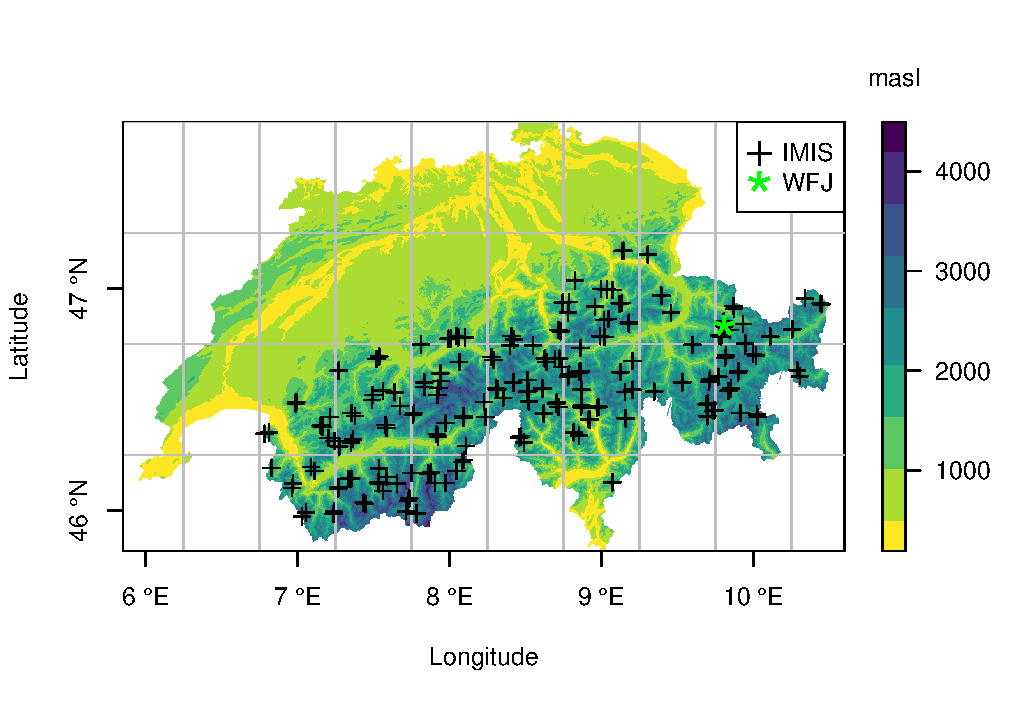
\includegraphics[width=18cm]{"plots/F1_map3.pdf"}
\caption{Study domain map with CORDEX grid overlaid. IMIS snow depth evaluation stations and the Weissfluhjoch meteorological station where downscaled timeseries are evaluated are plotted.}
\end{figure*}
% /home/joel/manuscripts/qmap/paper_specific_code/overview_map.R

\begin{figure*}[t]
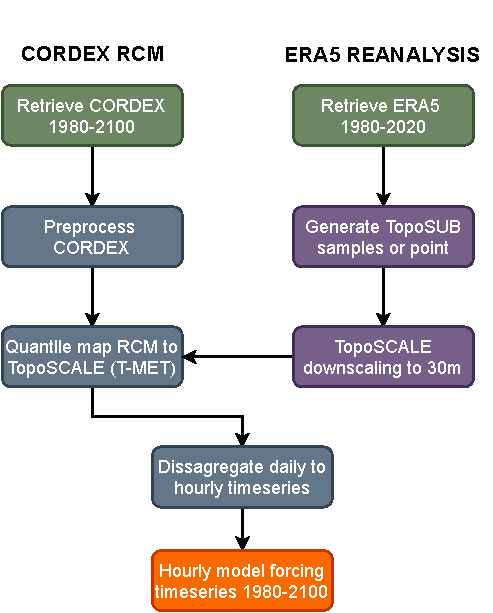
\includegraphics[width=10cm]{"plots/qmap_flow2.pdf"}
\caption{Flowchart of the main TopoCLIM processes.}
\label{fig:flow}
\end{figure*}
% edit here: https://drive.google.com/file/d/1MNuBP3NIaWRSfQtTEXi15nw0RqXEaTWY/view?usp=sharing


\begin{figure*}[t]
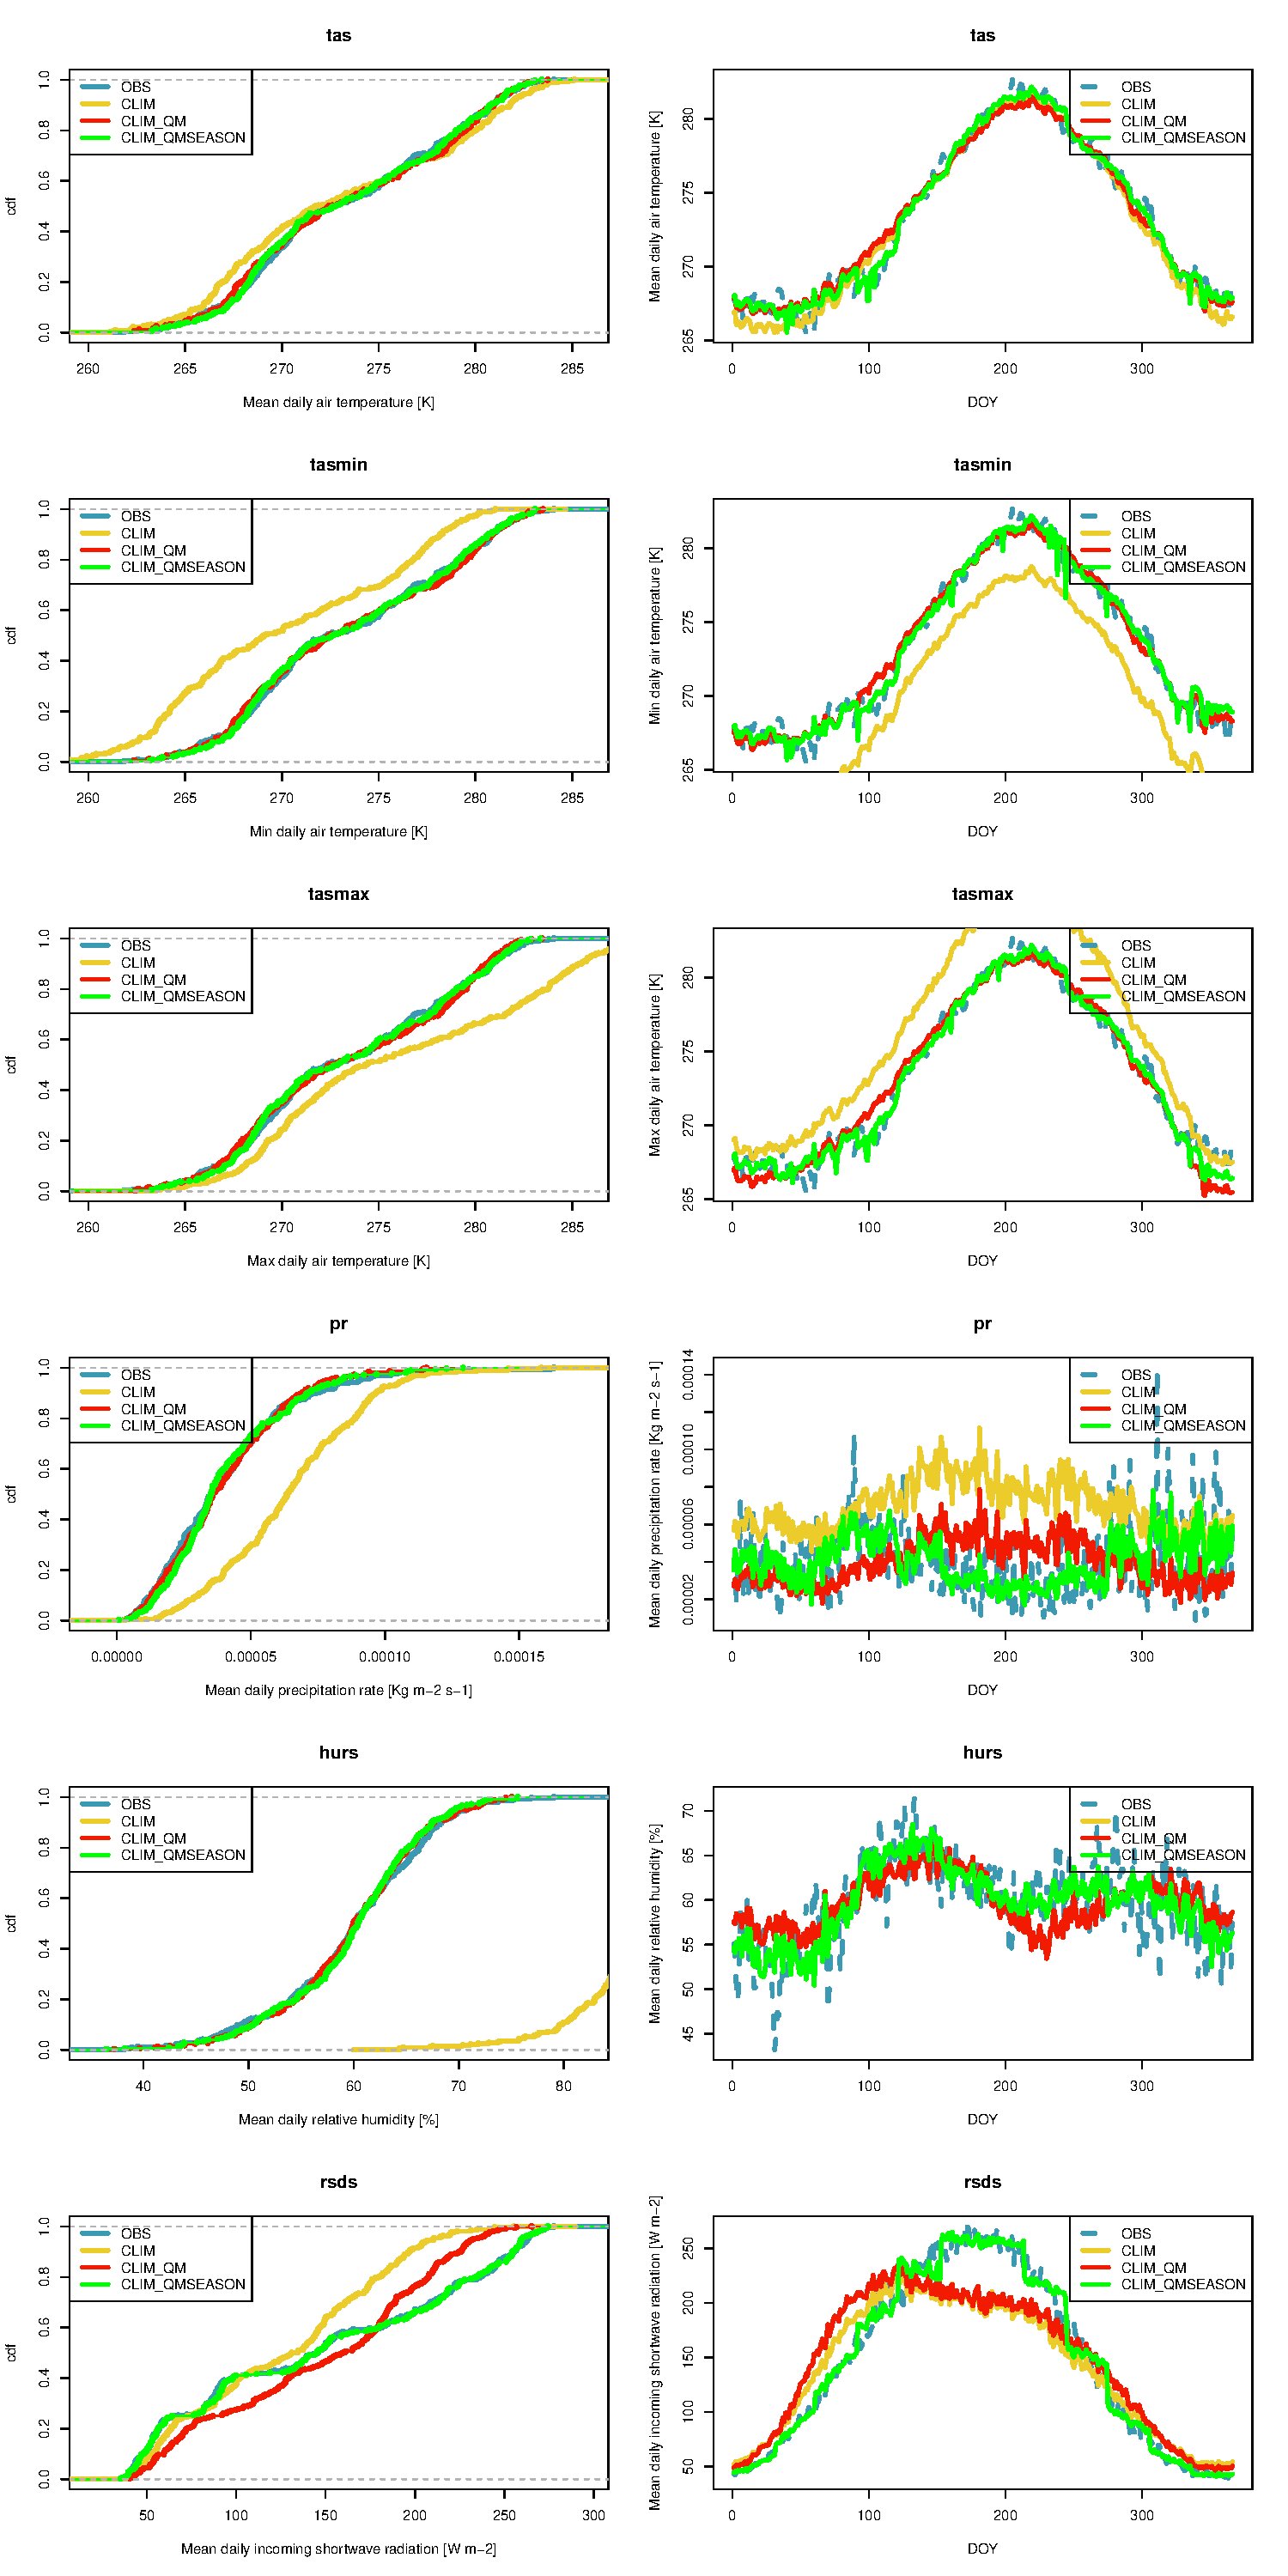
\includegraphics[width=10cm]{"plots/evalplot_singleModel_season.pdf"}
\caption{ Evaluation of the quantile mapping routine at the Weissfluhjoch station (T-MET) in standard mode "QM\_QM" (single parameter set) and "QM\_MONTH" seasonally varying parameter set. CLIM is the uncorrected CORDEX data. Shown are the cumulative density function over the period 1980-2005 (left panel) and seasonal distribution given as average by day of year (DOY) for the same period (right panel). }
\end{figure*}
% sample 189 from points run
% # settings for figure 3
% run in editor: tclim_hpc_qmap.py
% wd = '/home/joel/sim/qmap/tclim_points_paper/'
% tscale_sim_dir = "/home/joel/mnt/hyperion/sim/ch_points_paper/"
% cordex_dir= "/home/joel/sim/qmap/raw_cordex"
% starti=188
% endi = 189

% namelist = "/home/joel/src/FSM/nlst_tmapp.txt" # in src directory
% fsmexepath = "/home/joel/src/FSM/FSM" # version compiled on hyperion
% srcdir = "/home/joel/src/topoCLIM/"
% CORDEXPATH=cordex_dir+"/aresult_current/"


\begin{figure*}[t]
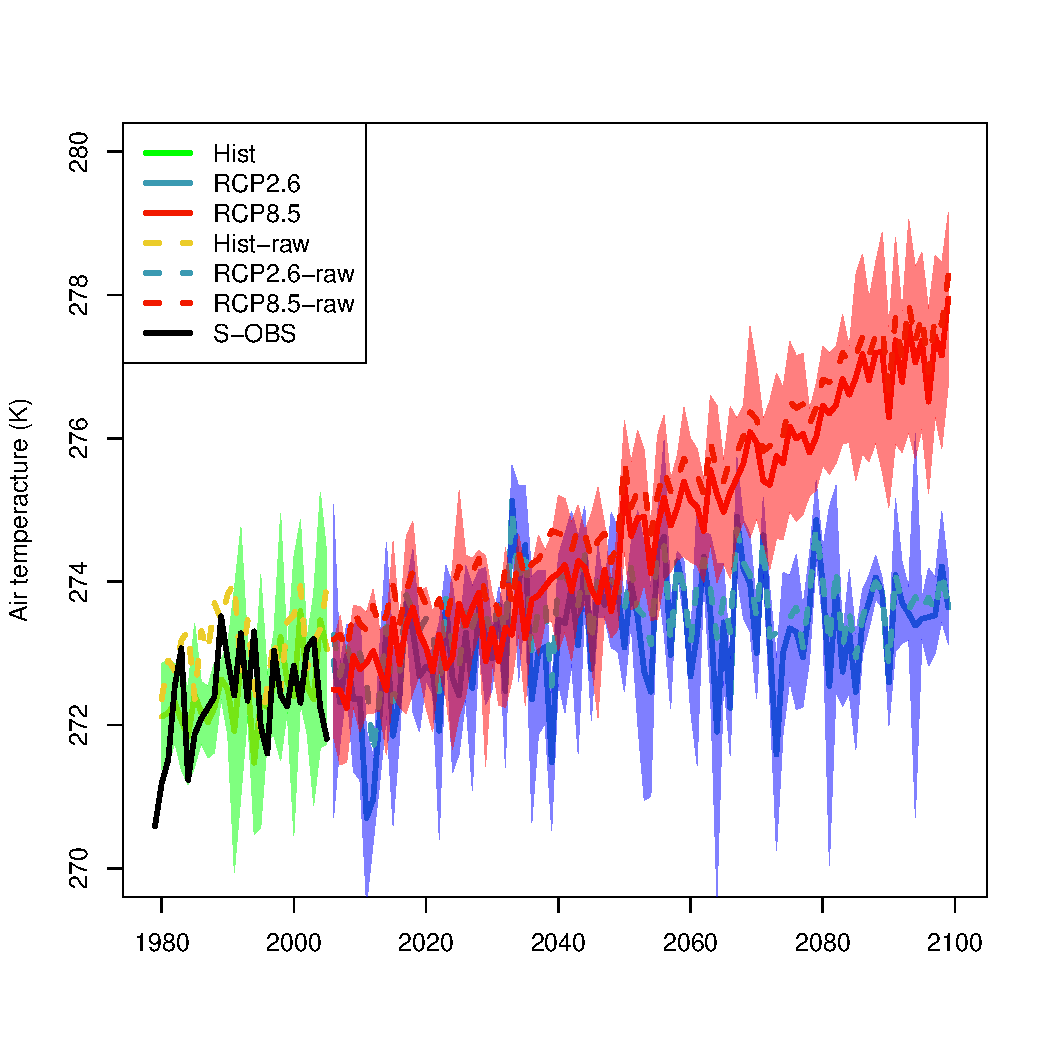
\includegraphics[width=10cm]{"plots/tasTS2.pdf"}
\caption{An example point-scale TopoCLIM product: Mean annual near surface air temperature at the Weissfluhjoch (2540 masl) showing corrected historical, RCP2.6 and RCP8.5 time series. Observations and uncorrected CORDEX data are also shown for comparison. The coloured envelopes indicate +/- 1 SD of the model spread and multi-modal mean is given by the bold line. }
\end{figure*}
%/home/joel/sim/qmap/PAPER_RESULTS/wfj_eval/stscale_189_1D/tasTS2.pdf



\begin{figure*}[t]
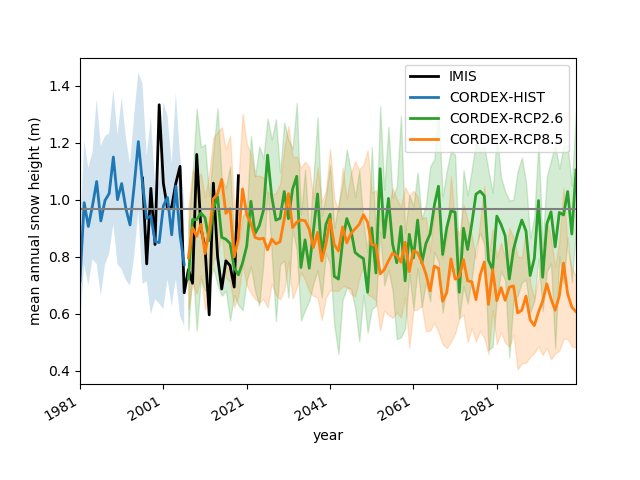
\includegraphics[width=12cm]{"plots/wfj_snow_TS2.png"}
\caption{An example point-scale TopoCLIM product: Mean annual snow depth (m) ensemble at the Weissfluhjoch (2540m asl) for historical and future RCP scenarios. Observation from WFJ2 are given in black. Ensemble means are indicated by solid line and long term average over the plotted historical period (1980-2006) is given by the horizontal line. Observations lie within the ensemble spread, indicating that the bias correction method works satisfactorily }
\end{figure*}

\begin{figure*}[t]

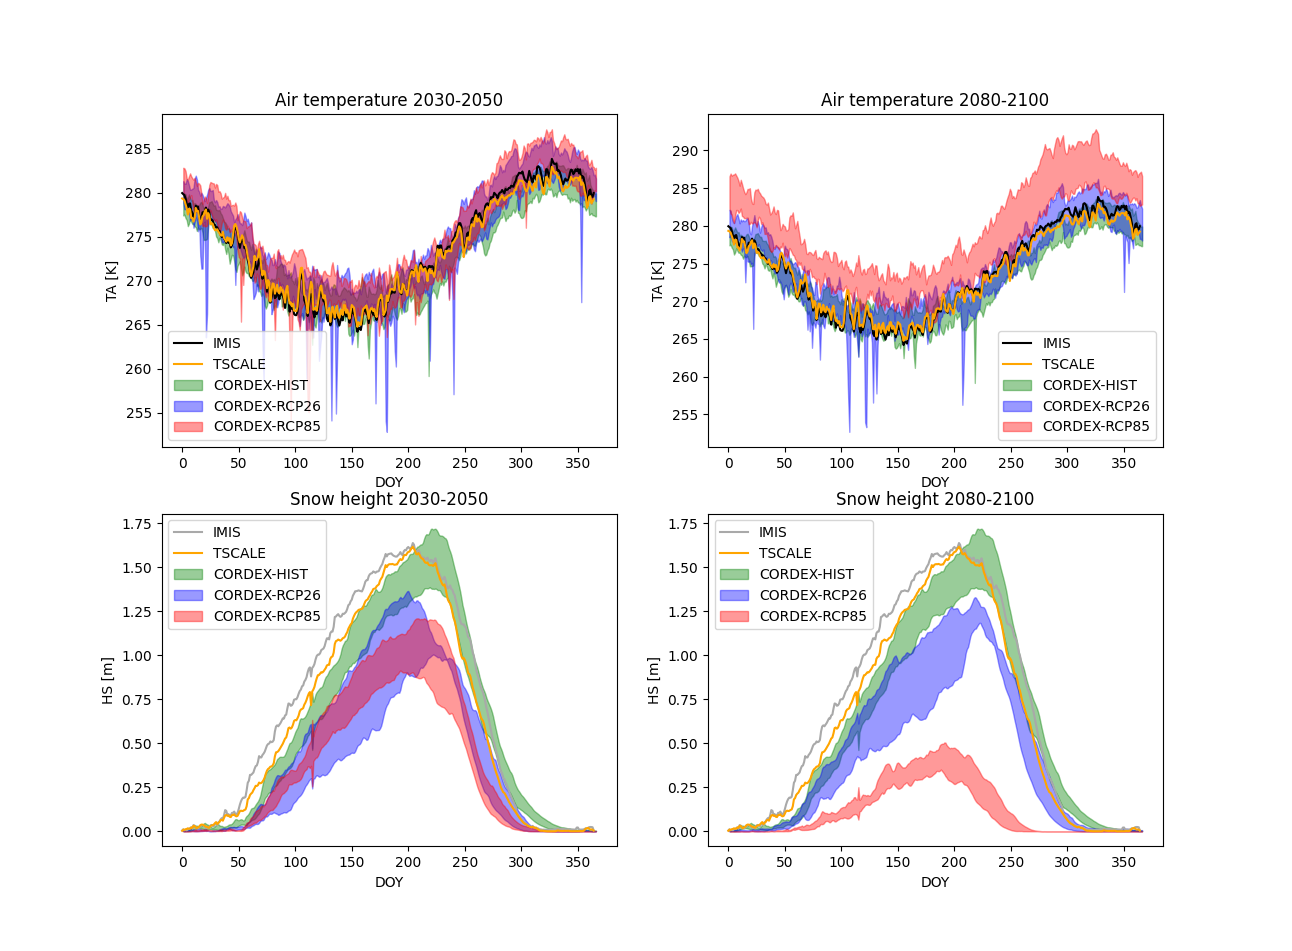
\includegraphics[width=18cm]{"plots/imis-4panel_V2.png"}
\caption{Large scale evaluation of the scheme: Mean DOY air temperature and snow height across all IMIS stations (IMIS) is compared to the same data generated by the TopoSCALE downscaling of ERA5 (TSCALE) and TopoCLIM downscaled CORDEX data for historical period (1980-2006) and scenarios RCP2.6/8.5 for near (2040-2060) and far future periods (2080-2100). The full width of model ensemble is represented by the shading. Note TSCALE and IMIS have the same time-frame (variable by station between 1996-2020) and therefore directly comparable, but only partially overlaps with the CORDEX HISTORICAL period and therefore is intended for visual comparison only. }
\end{figure*}

% for these models:
% x-special/nautilus-clipboard
% copy
% file:///home/joel/sim/qmap/raw_cordex/aresult/ICHEC-EC-EARTH_RCP2.6_r12i1p1_KNMI-RACMO22E_v1__TS_SCAL.nc
% file:///home/joel/sim/qmap/raw_cordex/aresult/ICHEC-EC-EARTH_RCP8.5_r1i1p1_KNMI-RACMO22E_v1__TS_SCAL.nc
% file:///home/joel/sim/qmap/raw_cordex/aresult/ICHEC-EC-EARTH_historical_r1i1p1_KNMI-RACMO22E_v1__TS_SCAL.nc

%merge_map.R
\begin{figure*}[t]
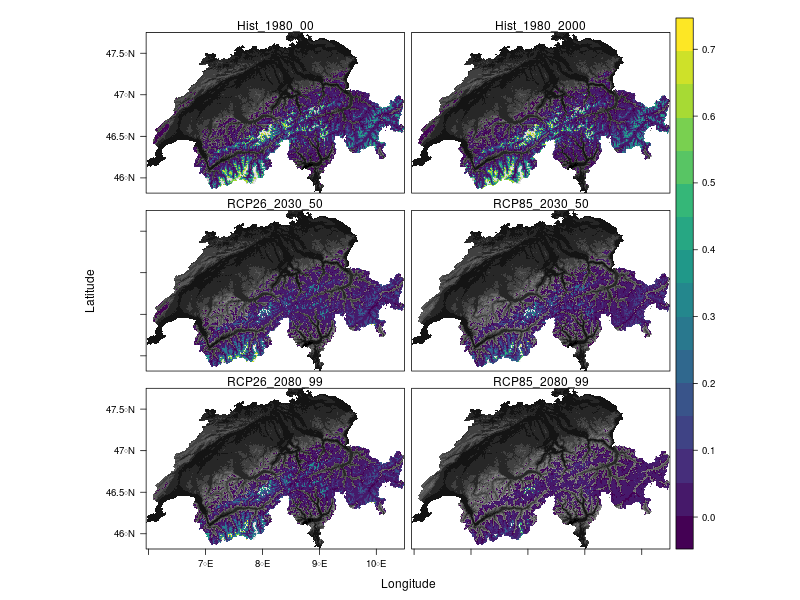
\includegraphics[width=20cm]{"plots/swe.png"}
\caption{Example TopoCLIM climate change maps: Mean snow depth (m) for RCP2.6 and RCP8.5 (columns) and time periods HIST, NEAR and FAR (rows). Non-seasonal snow-pack (does not melt in an annual cycle) is masked out and assumed to represent climatological glacier accumulation zones (ice surface fluxes are not modelled). These correspond well to existing glacier extent in period HIST. }
\end{figure*}

%\begin{figure*}[t]
%\includegraphics[width=18cm]{"plots/gst.png"}
%\caption{}
%\end{figure*}

\begin{figure*}[t]
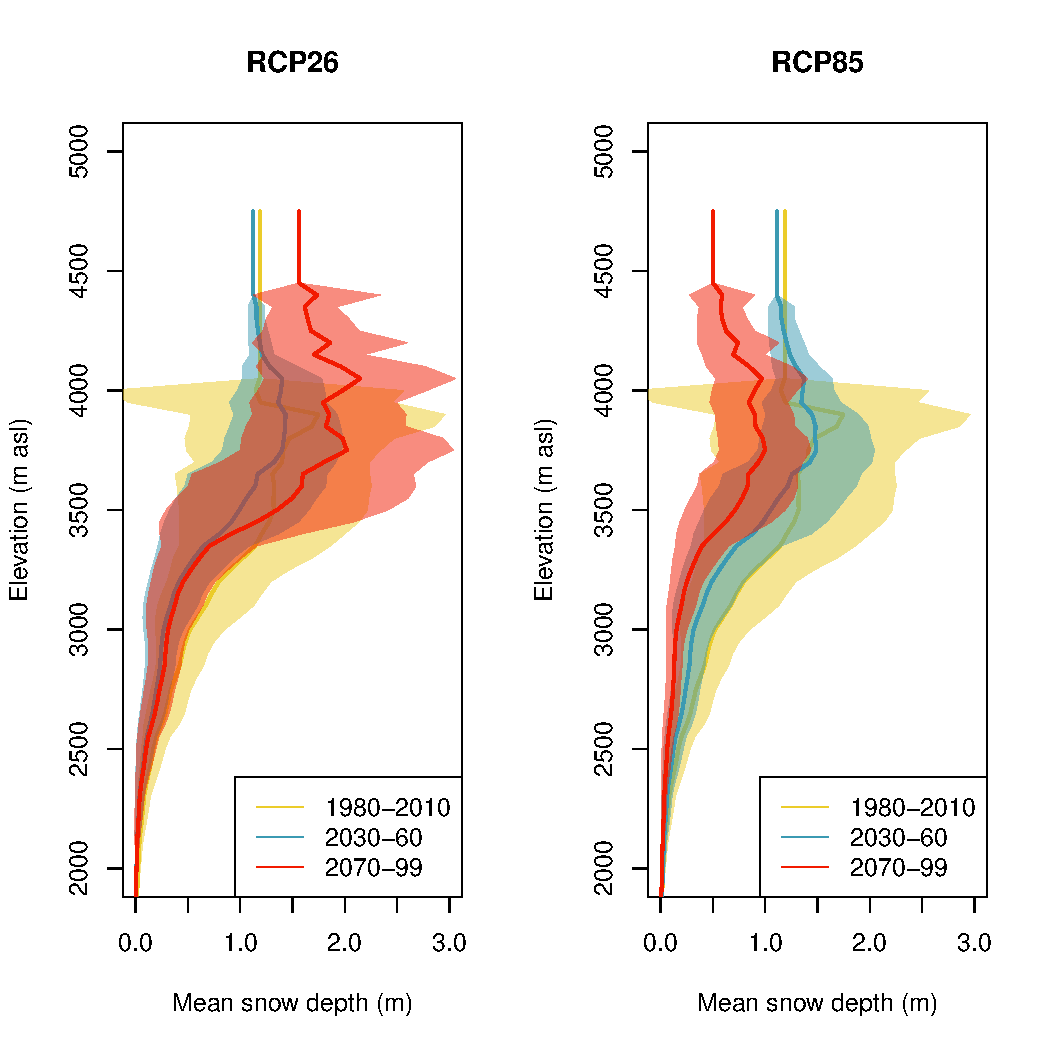
\includegraphics[width=18cm]{"plots/hypsometry_HS.pdf"}
\caption{Hypsometry of snow depth over the Swiss Alps for RCP2.6, RCP8.5 for periods HIST, NEAR and FAR. Data comes from the ensemble mean, shading gives +/- 1 standard deviation of values in each elevation band. Solid tail at top of plots represents glacier pixels which are masked in Figure X. This demonstrates the rising ELA of glaciers over the 21st century in all RCP's and extension of seasonal snow into the former glacier zones. }
\end{figure*}

%https://www.eea.europa.eu/data-and-maps/indicators/mountain-permafrost-1/assessment-1
%Projected change in sustainable near-surface permafost for four representative concentration pathways (RCP) based on the CMIP5 model ensemble. Soild lines show the model mean. For the highest and lowest RCP, uncertainty intervals comprising one standard deviation are also shown. Note that the projected reduction is for sustainable near-surface permafrost; it does not imply that deeper permafrost will disappear at a similar rate.https://www.overleaf.com/project/5efc7343d82afb000101eb21



%
%
 \clearpage
%%% TABLES
%%%
 \begin{table}[t]
 \begin{center}
% \begin{sidewaystable*}[t]
 \caption{CORDEX variables used in this study, together with the Climate and Forecast Conventions (CF) standard name .}
 \begin{tabular}{l l l l l }
\\[-1.8ex]\hline 
\hline \\[-1.8ex]
 output variable name  &units&timestep  & long\_name  &CF standard\_name \\
  \hline
 tas  &K&3  & Near-Surface Air Temperature  &air\_temperature  \\
 pr & kg m-2 s-1&3  &Precipitation  &precipitation\_flux \\
 ps & Pa&3  &Surface Air Pressure  &surface\_air\_pressure  \\
 hurs & \%&3    &Near-Surface Relative  &Humidity relative\_humidity \\
 rsds  &W m-2&3  & Surface Downwelling Shortwave Radiation & surface\_downwelling\_shortwave\_flux\_in\_air   \\
rlds  &W m-2&3 & Surface Downwelling Longwave Radiation & surface\_downwelling\_longwave\_flux\_in\_air\\
uas  &m s-1&6 &Eastward  Near-Surface Wind &eastward\_wind  \\
vas &m s-1&6 &Northward  Near-Surface Wind &northward\_wind \\

 \hline  
 \end{tabular}
 \label{tab:01}
% \end{sidewaystable*}
 \end{center}
\end{table}


% Table created by stargazer v.5.2.2 by Marek Hlavac, Harvard University. E-mail: hlavac at fas.harvard.edu
% Date and time: Fr, Jul 03, 2020 - 12:27:21
\begin{table}[!htbp] \centering 
  \caption{} 
  \label{} 
\begin{tabular}{@{\extracolsep{5pt}} ccccc} 
\\[-1.8ex]\hline 
\hline \\[-1.8ex] 
 & OBS & Hist & Hist\_QMAP & Hist\_QMAPSEASON \\ 
\hline \\[-1.8ex] 
MEAN & $0.170$ & $0.240$ & $0.170$ & $0.170$ \\ 
R-COR & $-$ & $$-$0.090$ & $$-$0.100$ & $0.210$ \\ 
RMSE & $-$ & $0.180$ & $0.130$ & $0.110$ \\ 
\hline \\[-1.8ex] 
\end{tabular} 
\end{table}

% get more models by accepting specific humidity and rcp 45

\begin{table}[!htbp] \centering 
  \caption{CORDEX model chains used in this study.} 
  \label{} 
\begin{tabular}{@{\extracolsep{5pt}} lllll} 
\\[-1.8ex]\hline 
\hline \\[-1.8ex] 
GCM&RCM&Scenario&Ensemble&Version \\ 
\hline \\[-1.8ex] 

 CCCma-CanESM2&SMHI-RCA4&RCP8.5&r1i1p1&v1 \\ 
 CNRM-CERFACS-CNRM-CM5&CLMcom-CCLM5-0-6&RCP8.5&r1i1p1&v1 \\ 
 CNRM-CERFACS-CNRM-CM5&CLMcom-CCLM5-0-6&historical&r1i1p1&v1 \\ 
 CNRM-CERFACS-CNRM-CM5&SMHI-RCA4&historical&r1i1p1&v1 \\ 
 CNRM-CERFACS-CNRM-CM5&CNRM-ALADIN53&RCP8.5&r1i1p1&v1 \\ 
 CNRM-CERFACS-CNRM-CM5&HMS-ALADIN52&RCP8.5&r1i1p1&v1 \\ 
 CNRM-CERFACS-CNRM-CM5&CNRM-ALADIN53&historical&r1i1p1&v1 \\ 
 CNRM-CERFACS-CNRM-CM5&SMHI-RCA4&RCP8.5&r1i1p1&v1 \\ 
 CSIRO-QCCCE-CSIRO-Mk3-6-0&SMHI-RCA4&historical&r1i1p1&v1 \\ 
 CSIRO-QCCCE-CSIRO-Mk3-6-0&SMHI-RCA4&RCP8.5&r1i1p1&v1 \\ 
 ICHEC-EC-EARTH&CLMcom-CCLM5-0-6&RCP8.5&r12i1p1&v1 \\ 
 ICHEC-EC-EARTH&CLMcom-CCLM5-0-6&historical&r12i1p1&v1 \\ 
 ICHEC-EC-EARTH&KNMI-RACMO22E&historical&r1i1p1&v1 \\ 
 ICHEC-EC-EARTH&SMHI-RCA4&RCP8.5&r12i1p1&v1 \\ 
 ICHEC-EC-EARTH&KNMI-RACMO22E&RCP2.6&r12i1p1&v1 \\ 
 ICHEC-EC-EARTH&KNMI-RACMO22E&RCP8.5&r1i1p1&v1 \\ 
 ICHEC-EC-EARTH&SMHI-RCA4&RCP2.6&r12i1p1&v1 \\ 
 ICHEC-EC-EARTH&KNMI-RACMO22E&historical&r12i1p1&v1 \\ 
 IPSL-IPSL-CM5A-MR&SMHI-RCA4&historical&r1i1p1&v1 \\ 
 IPSL-IPSL-CM5A-MR&SMHI-RCA4&RCP8.5&r1i1p1&v1 \\ 
 MIROC-MIROC5&SMHI-RCA4&historical&r1i1p1&v1 \\ 
 MIROC-MIROC5&CLMcom-CCLM5-0-6&RCP8.5&r1i1p1&v1 \\ 
 MIROC-MIROC5&SMHI-RCA4&RCP2.6&r1i1p1&v1 \\ 
 MIROC-MIROC5&SMHI-RCA4&RCP8.5&r1i1p1&v1 \\ 
 MOHC-HadGEM2-ES&KNMI-RACMO22E&RCP8.5&r1i1p1&v2 \\ 
 MOHC-HadGEM2-ES&CLMcom-CCLM5-0-6&RCP8.5&r1i1p1&v1 \\ 
 MOHC-HadGEM2-ES&SMHI-RCA4&historical&r1i1p1&v1 \\ 
 MOHC-HadGEM2-ES&SMHI-RCA4&RCP2.6&r1i1p1&v1 \\ 
 MOHC-HadGEM2-ES&SMHI-RCA4&RCP8.5&r1i1p1&v1 \\ 
 MOHC-HadGEM2-ES&CLMcom-CCLM5-0-6&historical&r1i1p1&v1 \\ 
 MPI-M-MPI-ESM-LR&SMHI-RCA4&historical&r1i1p1&v1 \\ 
 NCC-NorESM1-M&SMHI-RCA4&RCP2.6&r1i1p1&v1 \\ 
 NCC-NorESM1-M&SMHI-RCA4&historical&r1i1p1&v1 \\ 
 NCC-NorESM1-M&SMHI-RCA4&RCP8.5&r1i1p1&v1 \\ 
 NOAA-GFDL-GFDL-ESM2M&SMHI-RCA4&historical&r1i1p1&v1 \\ 
 NOAA-GFDL-GFDL-ESM2M&SMHI-RCA4&RCP8.5&r1i1p1&v1 \\ 
MPI-M-MPI-ESM-LR&CLMcom-CCLM5-0-6&RCP8.5&r1i1p1&v1 \\ 

\hline \\[-1.8ex] 
\end{tabular} 
\end{table}


%%% TWO-COLUMN TABLE
%
%%t
%\begin{table*}[t]
%\caption{TEXT}
%\begin{tabular}{column = lcr}
%\tophline
%
%\middlehline
%
%\bottomhline
%\end{tabular}
%\belowtable{} % Table Footnotes
%\end{table*}
%
%%% LANDSCAPE TABLE
%
%%t
%\begin{sidewaystable*}[t]
%\caption{TEXT}
%\begin{tabular}{column = lcr}
%\tophline
%
%\middlehline
%
%\bottomhline
%\end{tabular}
%\belowtable{} % Table Footnotes
%\end{sidewaystable*}
%
%
%%% MATHEMATICAL EXPRESSIONS
%
%%% All papers typeset by Copernicus Publications follow the math typesetting regulations
%%% given by the IUPAC Green Book (IUPAC: Quantities, Units and Symbols in Physical Chemistry,
%%% 2nd Edn., Blackwell Science, available at: http://old.iupac.org/publications/books/gbook/green_book_2ed.pdf, 1993).
%%%
%%% Physical quantities/variables are typeset in italic font (t for time, T for Temperature)
%%% Indices which are not defined are typeset in italic font (x, y, z, a, b, c)
%%% Items/objects which are defined are typeset in roman font (Car A, Car B)
%%% Descriptions/specifications which are defined by itself are typeset in roman font (abs, rel, ref, tot, net, ice)
%%% Abbreviations from 2 letters are typeset in roman font (RH, LAI)
%%% Vectors are identified in bold italic font using \vec{x}
%%% Matrices are identified in bold roman font
%%% Multiplication signs are typeset using the LaTeX commands \times (for vector products, grids, and exponential notations) or \cdot
%%% The character * should not be applied as mutliplication sign
%
%
%%% EQUATIONS
%
%%% Single-row equation
%
%\begin{equation}
%
%\end{equation}
%
%%% Multiline equation
%
%\begin{align}
%& 3 + 5 = 8\\
%& 3 + 5 = 8\\
%& 3 + 5 = 8
%\end{align}
%
%
%%% MATRICES
%
%\begin{matrix}
%x & y & z\\
%x & y & z\\
%x & y & z\\
%\end{matrix}
%
%
%%% ALGORITHM
%
%\begin{algorithm}
%\caption{...}
%\label{a1}
%\begin{algorithmic}
%...
%\end{algorithmic}
%\end{algorithm}
%
%
%%% CHEMICAL FORMULAS AND REACTIONS
%
%%% For formulas embedded in the text, please use \chem{}
%
%%% The reaction environment creates labels including the letter R, i.e. (R1), (R2), etc.
%
%\begin{reaction}
%%% \rightarrow should be used for normal (one-way) chemical reactions
%%% \rightleftharpoons should be used for equilibria
%%% \leftrightarrow should be used for resonance structures
%\end{reaction}
%
%
%%% PHYSICAL UNITS
%%%
%%% Please use \unit{} and apply the exponential notation


\end{document}
